\chapter{Resoconto attività di verifica}

\section{Metriche fino allo Sprint 12}

  \subsection{Verifica documenti}
    \subsubsection{Indice di Gulpease}
    \begin{figure}[H]
      \centering
      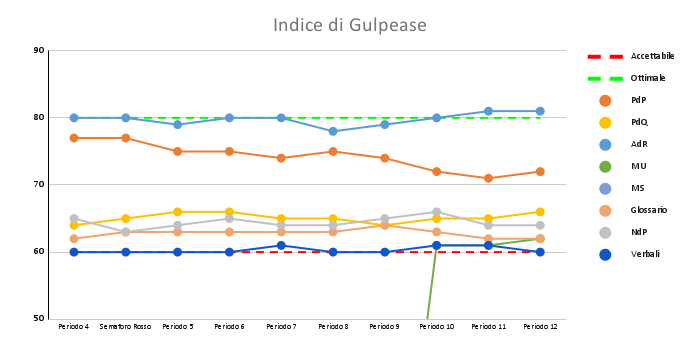
\includegraphics[scale=0.60]{Indice di Gulpease.png}
      \caption{Indice di Gulpease per documento per periodo}
    \end{figure}

  \subsection{Verifica del software}
    \subsubsection{Tempo medio di risposta}
    \begin{figure}[H]
      \centering
      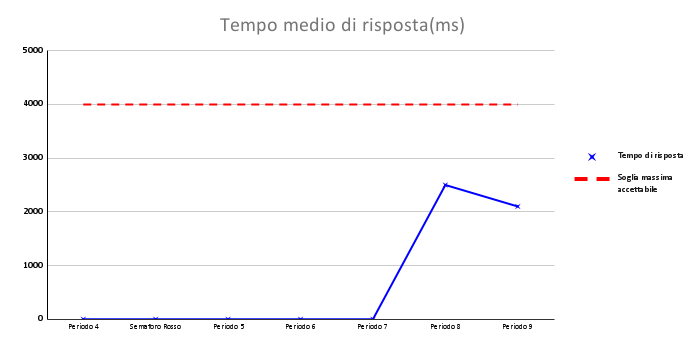
\includegraphics[scale=0.60]{Tempo medio di risposta(ms).png}
      \caption{Tempo medio di risposta dell'applicazione(ms)}
    \end{figure}


  \subsection{Verifica dei processi}
    \subsubsection{Estimated at Completion}
    \begin{figure}[H]
      \centering
      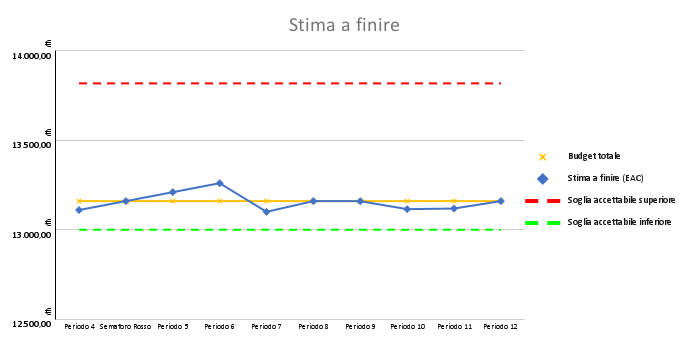
\includegraphics[scale=0.60]{Stimaafinire2.png}
      \caption{Valore stimato per la realizzazione del progetto}
    \end{figure}

    \subsubsection{Actual Cost e Estimate to Complete}
    \begin{figure}[H]
      \centering
      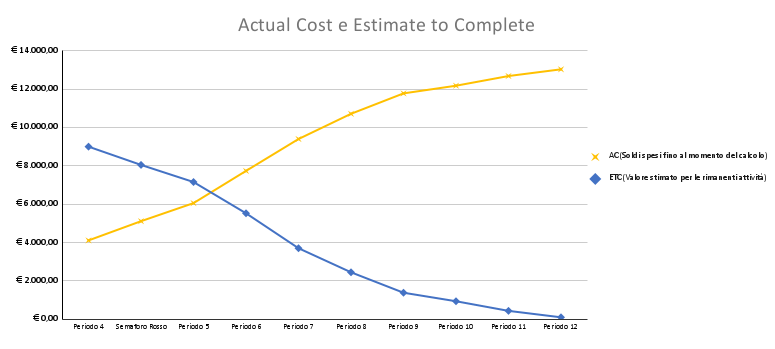
\includegraphics[scale=0.60]{Actual Cost e Estimate to Complete.png}
      \caption{Costo effettivamente sostenuto e valore stimato per la realizzazione delle rimanenti attività}
    \end{figure}

    \subsubsection{Earned Value e Planned Value}
    \begin{figure}[H]
      \centering
      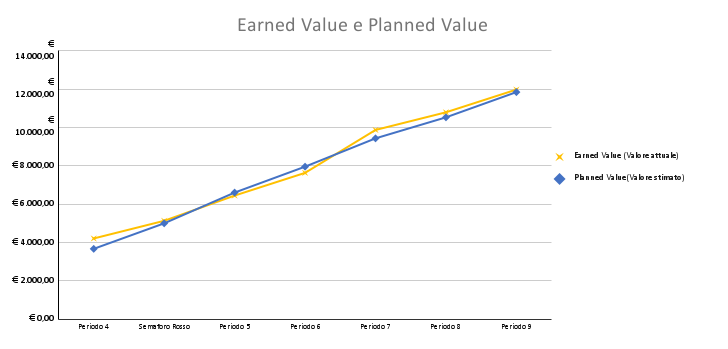
\includegraphics[scale=0.60]{Earned Value e Planned Value.png}
      \caption{Valore delle attività realizzate e costo pianificato per realizzare le rimanenti}
    \end{figure}

    \subsubsection{Schedule Variance e Budget Variance}
    \begin{figure}[H]
      \centering
      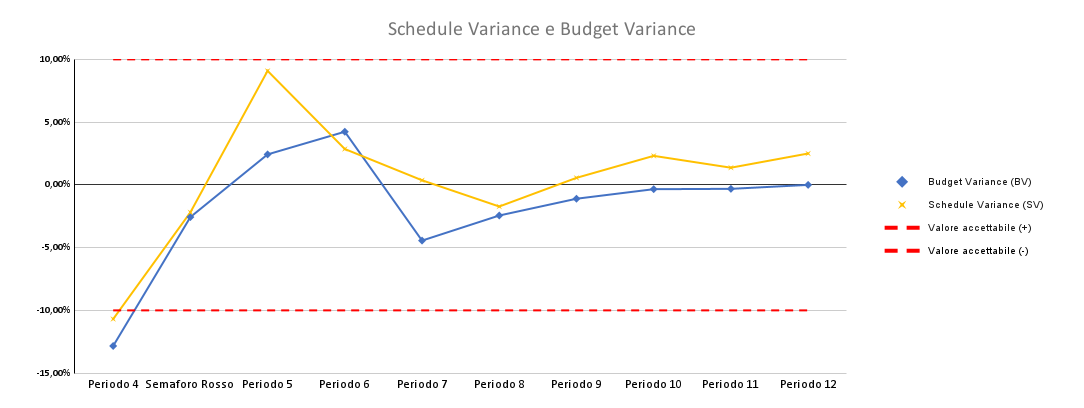
\includegraphics[scale=0.48]{Schedule Variance e Budget Variance.png}
      \caption{Schedule Variance e Budget Variance per incremento}
    \end{figure}

    \subsubsection{Copertura e stabilità dei requisiti}
    \begin{figure}[H]
      \centering
      \includegraphics[scale=0.60]{Indice di Stabilità dei Requisiti e Requisiti Obbligatori Soddisfatti.png}
      \caption{Percentuale di copertura e stabilità dei requisiti}
    \end{figure}

    \subsubsection{Metriche soddisfatte}
    \begin{figure}[H]
      \centering
      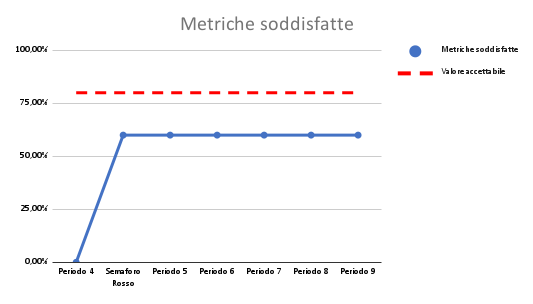
\includegraphics[scale=0.60]{Metriche soddisfatte.png}
      \caption{Percentuale di metriche di qualità soddisfatte}
    \end{figure}

    \subsubsection{Facilità di utilizzo}
    \begin{figure}[H]
      \centering
      \includegraphics[scale=0.60]{Facilità di utilizzo(click).png}
      \caption{Facilità di utilizzo espressa in click}
    \end{figure}

    \subsubsection{Comprensibilità codice}
    \begin{figure}[H]
      \centering
      \includegraphics[scale=0.48]{Comprensibilità codice.png}
      \caption{Percentuale di Comprensibilità del codice}
    \end{figure}

    \subsubsection{Browser supportati}
    \begin{figure}[H]
      \centering
      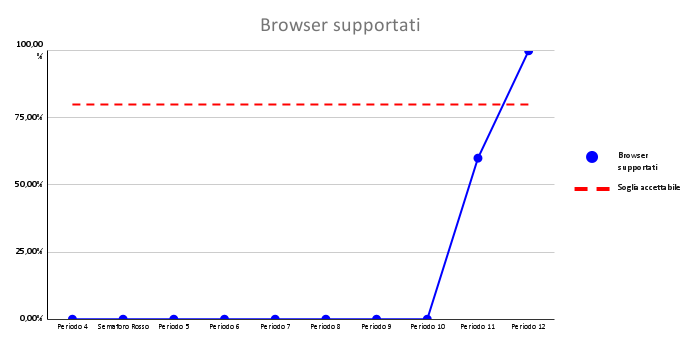
\includegraphics[scale=0.60]{Browser supportati.png}
      \caption{Percentuale di browser supportati sul totale}
    \end{figure}

    \subsubsection{Code coverage e percentuale di test superati/falliti}
    \begin{figure}[H]
      \centering
      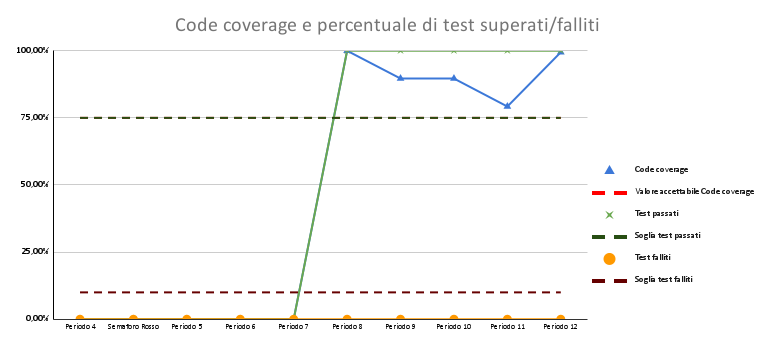
\includegraphics[scale=0.60]{Code coverage e percentuale di test superati_falliti2.png}
      \caption{Copertura del codice e percentuale di test superati e falliti per incremento. In questo grafico non sono presenti i file drawer.}
    \end{figure}

    \subsubsection{Copertura dei test}
    \begin{figure}[H]
      \centering
      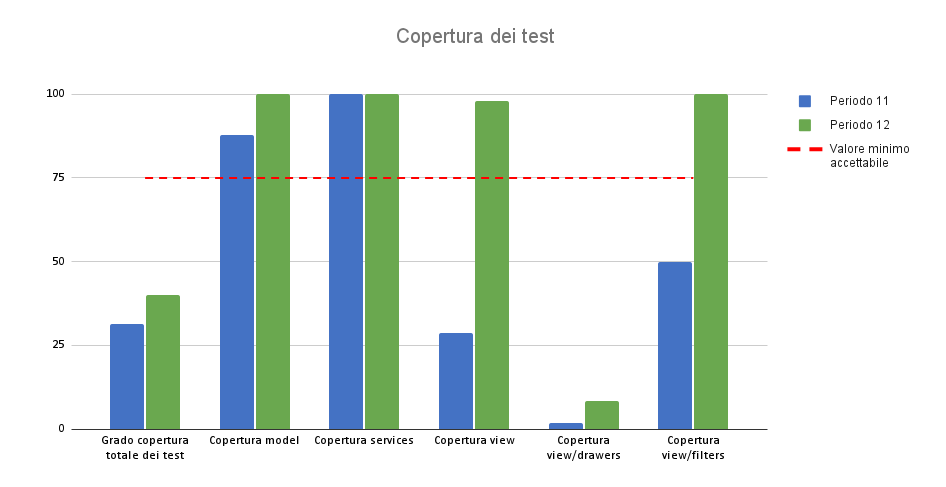
\includegraphics[scale=0.50]{Copertura dei test.png}
      \caption{Copertura offerta dai test per ogni componente}
    \end{figure}

    \begin{figure}[H]
      \centering
      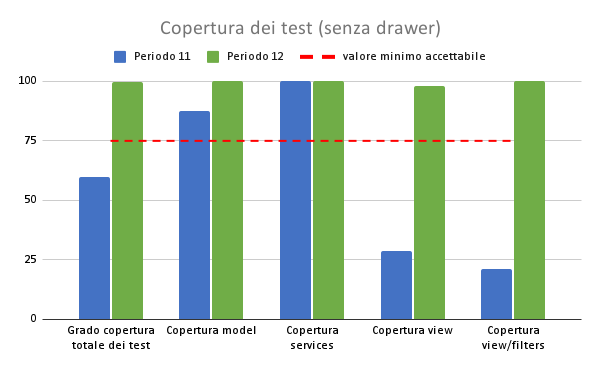
\includegraphics[scale=0.60]{Copertura dei test (senza drawer).png}
      \caption{Copertura offerta dai test trascurando la componente "drawer"}
    \end{figure}

    \subsubsection{Numero di test per componente}
    \begin{figure}[H]
      \centering
      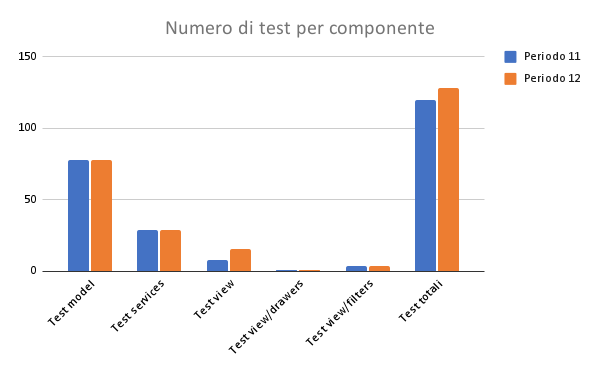
\includegraphics[scale=0.60]{Numero di test per componente.png}
      \caption{Numero di test per componente}
    \end{figure}

    \subsubsection{Test sul totale per ogni componente}
    \begin{figure}[H]
      \centering
      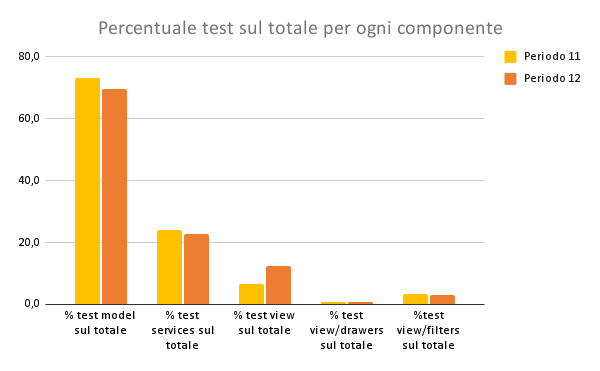
\includegraphics[scale=0.60]{Percentuale test sul totale per ogni componente.png}
      \caption{Percentuale di test sul totale per ogni componente}
    \end{figure}
